% !TEX encoding = UTF-8
% !TEX TS-program = pdflatex
% !TEX root = ../tesi.tex
% !TEX spellcheck = it-IT

\section{DBSCAN}
L'idea \lq\lq chiave\rq\rq dell'algoritmo DBSCAN\cite{Ester96adensity} è che ciascun elemento di un cluster debba avere un vicinato entro un certo raggio $\epsilon$ (Eps)  che contenga almeno un numero minimo di punti (MinPts). Questo algoritmo, in altre parole, stima la \emph{densità} di ciascun punto, per mezzo della cardinalità del suo \lq\lq vicinato\rq\rq entro un raggio predefinito $Eps$. Un punto sarà definito come \emph{core-object} se la densità del suo vicinato supera una data soglia $MinPts$.
Un punto $q$ si dice \lq\lq directly density-reachable\rq\rq  da un core-object $p$, se $q$ ricade nell'eps-vicinato di $p$.
La chiusura transitiva  di questa proprietà, è detta density-reachability. Due punti $p$ e $q$ si diranno invece, \emph{density-connected}, se esiste un terzo oggetto $o$ dal quale entrambi sono density-reachable. Grazie a quest'ultima proprietà è possibile definire un cluster, ovvero come un insieme di oggetti densamente connessi che è massimale rispetto alla proprietà di density-reachability. Il noise, invece, sarà dato dall'insieme di punti che non appartengono a nessuno di questi cluster.  In seguito verranno date le definizioni in maniera più formale:
 %defizioni di DBSCAN
\begin{definizione}[directly density-reachable]
\label{def:ddr}
Un oggetto $p$ si dice 	\emph{directly-density-reachable} da un oggetto $q$ rispetto ai parametri $Eps$ ed $MinPts$ nell'insieme di oggetti $D$ se:
\begin{enumerate}
\item $p \in Neigh_{eps(Q)}$
\item $|Neigh_{eps(Q)}| \ge MinPts$
\end{enumerate}
\end{definizione}
\begin{definizione}[density-reachable]
\label{def:dr} 
Un oggetto   $p$ si dice 	\emph{"density-reachable"} da un oggetto $q$ rispetto ai parametri $Eps$ ed $MinPts$ nell'insieme di oggetti $D$, e si  indica con \emph{$p>_{D}q$}, se esiste una catena di oggetti: $p_1,\dots,p_n$, $p_1=p p_n=q$ tali che:  $p_{i} \in D  \land p_{i+1}$ è \emph{directly-density-reachable} da $p_{i}$
\end{definizione}
Questa relazione è l'estensione canonica della relazione Directly-density-reachability, inoltre è una relaione transitiva ma non simmetrica. Sebbene non sia simmetrica, vi sono delle zone nell'isnieme $D$, in cui questa relazione è simmetrica ovvero  per quegli oggetti $o$ nell insieme per cui $|N_{eps(o)}| \ge MinPts$. Due oggetti \emph{border}, ovvero due oggetti che giacciono sul confine di un cluser, probabilmente non saranno density-reachable fra loro in quanto non ci sono abbastanza oggetti nel loro vicinato. Tuttavia, ci sarà necessariamente, un terzo oggetto nel cluster dal quale entrambi questi  oggetti border saranno density-reachable.
%figura esempio
\begin{figure}
\centering
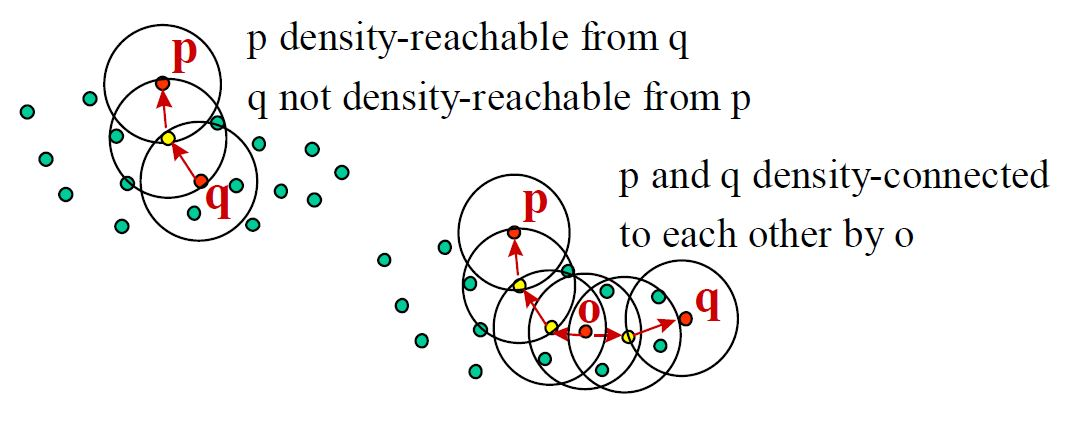
\includegraphics[width=0.6\textwidth]{density-reachable}
\caption{Density Reachability e Density Connectivity}
\label{fig:dens-reach}
\end{figure}
%density connected def
\begin{definizione}[density-connected]
\label{def:dc}
Un oggetto $p$ si dice 	\emph{"density-connected"} da un oggetto $q$ wrt $Eps$ ed $MinPts$ nell'insieme di oggetti $D$ se esiste un oggetto $o \in D$  tale che sia $p$ che $q$ siano \emph{ density reachable} da $o$. La relazione di density-connectivity è simmetrica, la figura \ref{fig:dens-reach} mostra la le definizioni su descritte in uno spazio bi-dimensionale. 
\end{definizione} 
Proprio grazie alla proprietà di density connectivity, si potrà dare la definizione di cluster ovvero un insieme massimale di oggetti \lq\lq densamente connessi\rq\rq.
%cluster def
\begin{definizione}[cluster]
\label{def:cluster}
Sia $D$ un insieme di oggetti.
Si defnisce \emph{\lq\lq cluster\rq\rq}  $C$,  wrt $Eps$ ed $MinPts$ nell'insieme di oggetti $D$,
un sottoniseme non vuoto di $D$, che soddisfa le seguenti condizioni :
\begin{enumerate}
\item \emph{Massimalità}: $\forall p,q\in D$, se $p \in C \land q>_{D}p$ wrt MinPts e Eps, 
allora anche $q \in C  $

\item \emph{Connettività}: $\forall p,q\in C$, $p$ è \emph{"density-connected"} a $q$  wrt MinPts e Eps

\end{enumerate}
 
\end{definizione} 


%def noise
\begin{definizione}[noise]
\label{def:noise}
Siano $C_1,\dots,C_k$ tutti i cluster wrt Eps e , ovvero come un insieme di oggetti densamente connessi che è massimale rispetto MinPts in $D$. Si definisce \emph{noise}  l'insieme di oggetti $D$ che non appartengono a nessun cluster $C_i$,
noise=$\lbrace p\in D | \forall i: p \notin C_i \rbrace $.
 
\end{definizione}
Questo algoritmo presenta due proprietà fondamentali che ne permettono una computazione efficiente:
\begin{enumerate}
\item Dato un qualsiasi core-object, l'insieme dei punti density reachable da tale punto (w.r.t Eps,MinPts) costituirà un cluster.
\item  Si consideri un cluster $C$, ciacun elemento di C è density-reachable da  un ogni core-object in C. Ciascun cluster sarà quindi, univocamente identificato da uno qualsiasi dei suoi core-object.
\end{enumerate}

L'algoritmo di DBSCAN, al fine di creare un cluster,parte da un punto arbitrario $p$ e ritrova tutti i punti da esso density-reachable rispetto ai parametri $Eps$ e $MinPts$, effettuando region-query \footnote{una region-query  di un punto $p$ è la ricerca dei punti che ricadono nel viciniato di $p$} prima per $p$ ed eventualmente per i vicini di p diretti ed indiretti.
Se l'oggetto $p$ è un core-object tale procura ci darà un cluster, altrimenti l'oggetto $p$ sarà considerato come NOISE, e si passerà al oggetto successivo. Se $p$ è un border-point sarà successivamente ri-etichettato quando, verrà considerato un core object dal quale $p$ è density reachable.
Le implementazioni classiche di DBSCAN fanno uso di indici spaziali come R-tree o X-tree, che consentono di ritrovare il viciniato di ciacun punto (region-query) in maniera efficiente $O(logn)$. Nel peggiore dei casi, DBSCAN visita ogni punto del dataset, ovvero esegue una region query per ciascun punto, ciò determina una complessità $0(n^2)$  dove $n$ rappresenta il numero di punti nel dataset. Se si utilizza una struttura indicizzata come un R-tree, è possibile passare ad una coplessità $0(nlogn)$ . 
Tali strutture indicizzate però, non riescono a scalare all'aumentare della dimensionalità dei dati: la performance delle region query passa da  O(logn)to O(n), facendo degenerare, cioè la complessità temporale di dbscan in $O(n^2)$ rendendo poco adatto questo algoritmo al problema del clustering dei tweets. Nel lavoro di Guo et al. \cite{4370588} vien proposto una variante dell'algoritmo DBSCAN che fa uso dell'LSH, al fine di ritrovare i nearest-neighbors di un punto, riducendo sensibilmente la complessità dell'algoritmo.
 
 %note dbscan
L'algoritmo DBSCAN riesce  a generare dei cluster anche con un elevata presenza di rumore. Inoltre grazie alla definizione di "density-connected"\ref{def:dc}, riesce ad identificare cluster di forme arbitrarie. Inoltre, a differenza di altri algoritmi come k-means, non necessita di conoscere a priori il numero di cluster. Tutte queste caratteristiche rendono questo algoritmo particolarmente interessante nella scoperta di cluster in questo lavoro di tesi poiché: i messaggi di un microblog come Twitter contengono un'alta percentuale di rumore, e nel task di event-detection non è possibile sapere a priori il numero di eventi.
\subsection{DBSCAN come ricerca di componenti connesse }
Il problema del clustering, può essere ricondotto al problema della ricerca di componenti connesse in un grafo.
In un grafo, una \emph{componente connessa} è un sotto-grafo in cui ogni coppia di vertici è connessa da un cammino, e il sottografo non è connesso  a nessun altro vertice  del grafo di partenza. Per ottenere una corrispondenza fra una  componente ed  un cluster secondo dbscan, sarà sufficiente far sì che per ogni coppia di punti  density-connected, esista un cammino che li colleghi.
\begin{figure}
    \centering
    \begin{subfigure}[b]{0.45\textwidth}
        \centering
        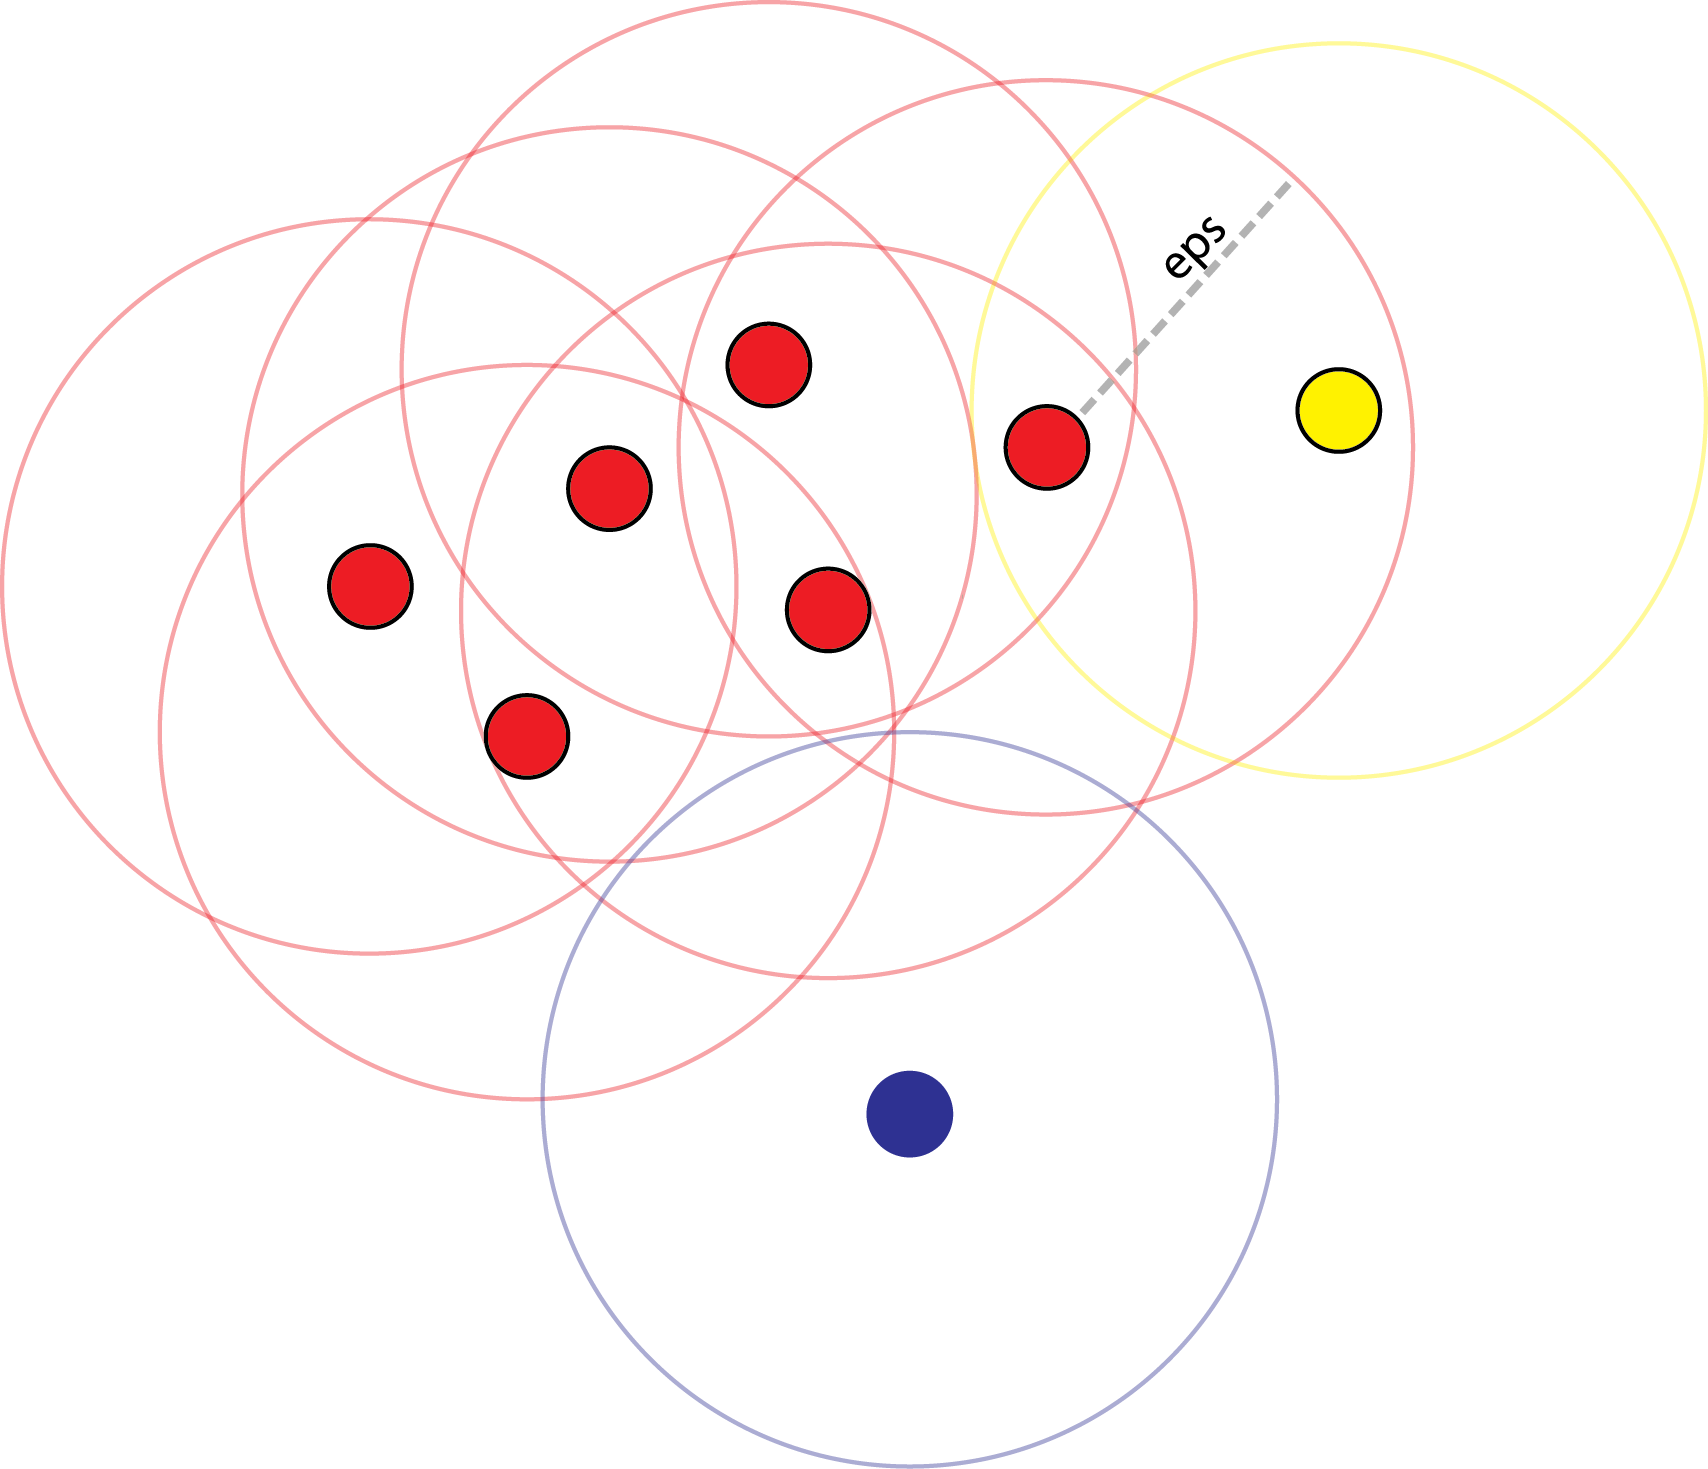
\includegraphics[width=\textwidth]{dbscanWithoutPaths}
       	\caption{ MinPts=3}
         \label{fig:densityConnectedObjects}
    \end{subfigure}
    \hfill
    \begin{subfigure}[b]{0.45\textwidth}
        \centering
        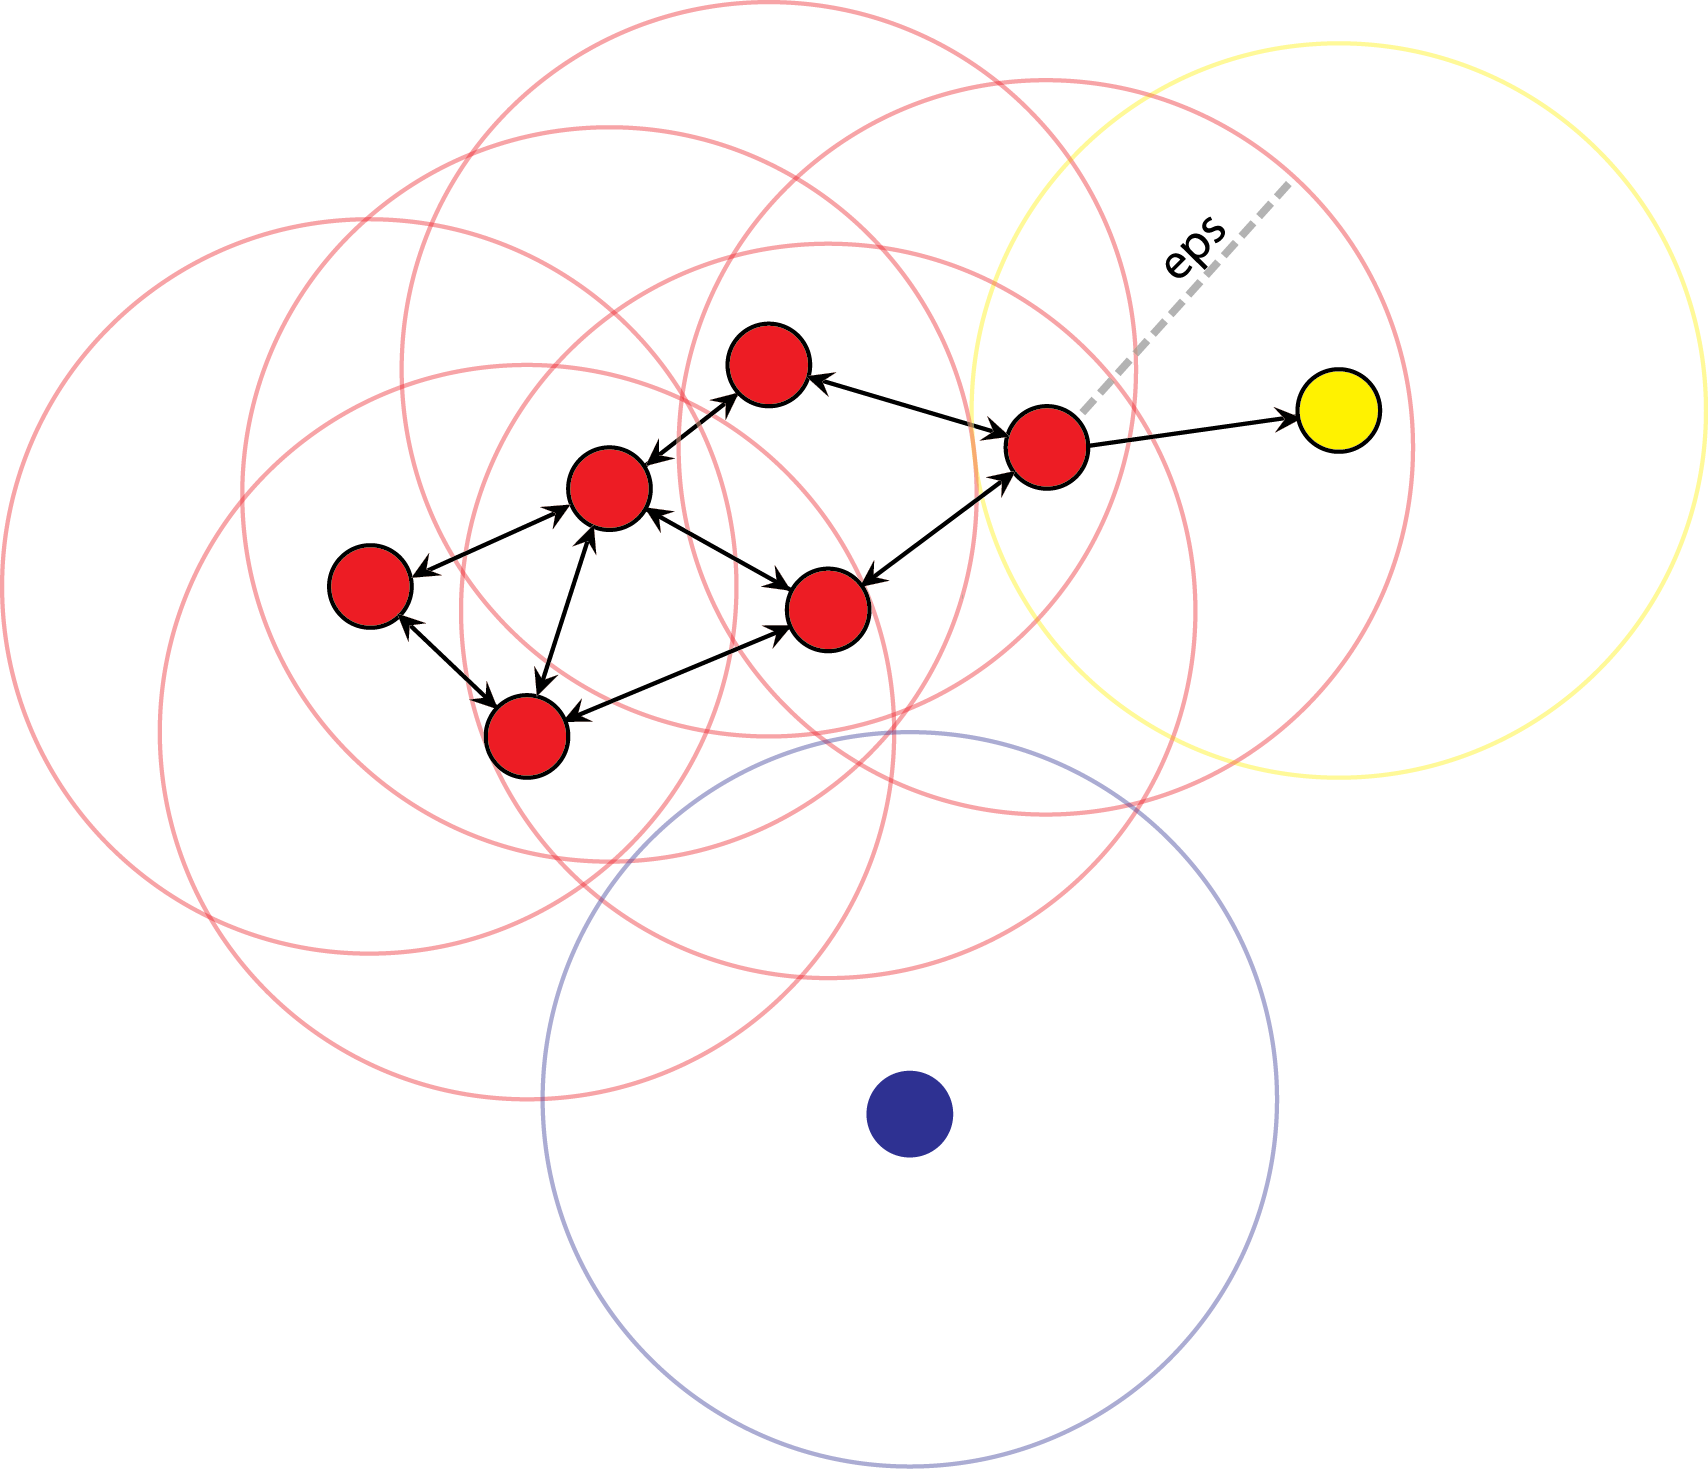
\includegraphics[width=\textwidth]{dbscanPaths}
        \caption{Esempio di grafo di densità}
         \label{fig:graphdensityConnectedObjects}
    \end{subfigure}
    \hfill
    \caption{rossi=core-objects, gialli=border,
    	blue=noise}
    \label{fig:dbscangraph}
\end{figure} 
In figura \ref{fig:graphdensityConnectedObjects} è mostrato come è possibile rappresentare un grafo-diretto a partire da connessioni di densità: per ogni coppia di oggetti di  directly density reachable $a,b$ con $a$ core-object,
verrà creato un arco $(a,b)$, se anche $b$ è un core object sarà creato un ulteriore arco da $b$ ad $a$ : $(b,a)$.
Talvolta però, un border-object può essere nel vicinato di più di un core-object anche appartenenti a cluster distinti, come mostrato in figura \ref{fig:dbscanGraphRevisited}. Se fossero lasciati entrambi gli archi verso il border-object, verrebbe identificata un'unica componente connessa. Lasciare questi archi renderebbe l'algoritmo molto più sensibile al rumore, poiché in tal un solo punto potrebbe determinare la fusione di più cluster.

Per evitare tali problematiche, bisogna costruire un grafo i cui nodi sono sono soltanto i \emph{core-objects}, e verrà aggiunto un arco fra due nodi solo se la loro distanza è minore di $eps$.  In maniera più formale il grafo è cosi definito:

$
G=(V,A) \:$ dove :

$ V= \lbrace x \in D \:| \: Card(Neigh_{eps(x)}) \ge MinPts\rbrace$


$ A= \lbrace (x,y) \in V \:| \: d(x,y) \le eps \rbrace$

A partire da questo grafo $G$ verranno identificate tutte le componenti connesse che corrispondo ai cluster, individiuati però solo a partire dai nodi cores. Bisognerà quindi eseguire un ulteriore step per assegnare gli oggetti border ad un cluster con cui sono connessi. L'algoritmo originale nel caso in cui un oggetto border   ricada nel vicinato di più core objects, ciascuno dei quali di un cluster differente, lo assegnerebbe in maniera  casuale ad uno di questi cluster. In questo caso è possibile adottare tre strategie diverse:
\begin{itemize}
\item scegliere in maniera casuale un cluster 
\item scegliere il cluster con cui il border object ha maggiore connettività 
\item scegliere il cluster più vicino al border object
\end{itemize}

\begin{figure}
\centering
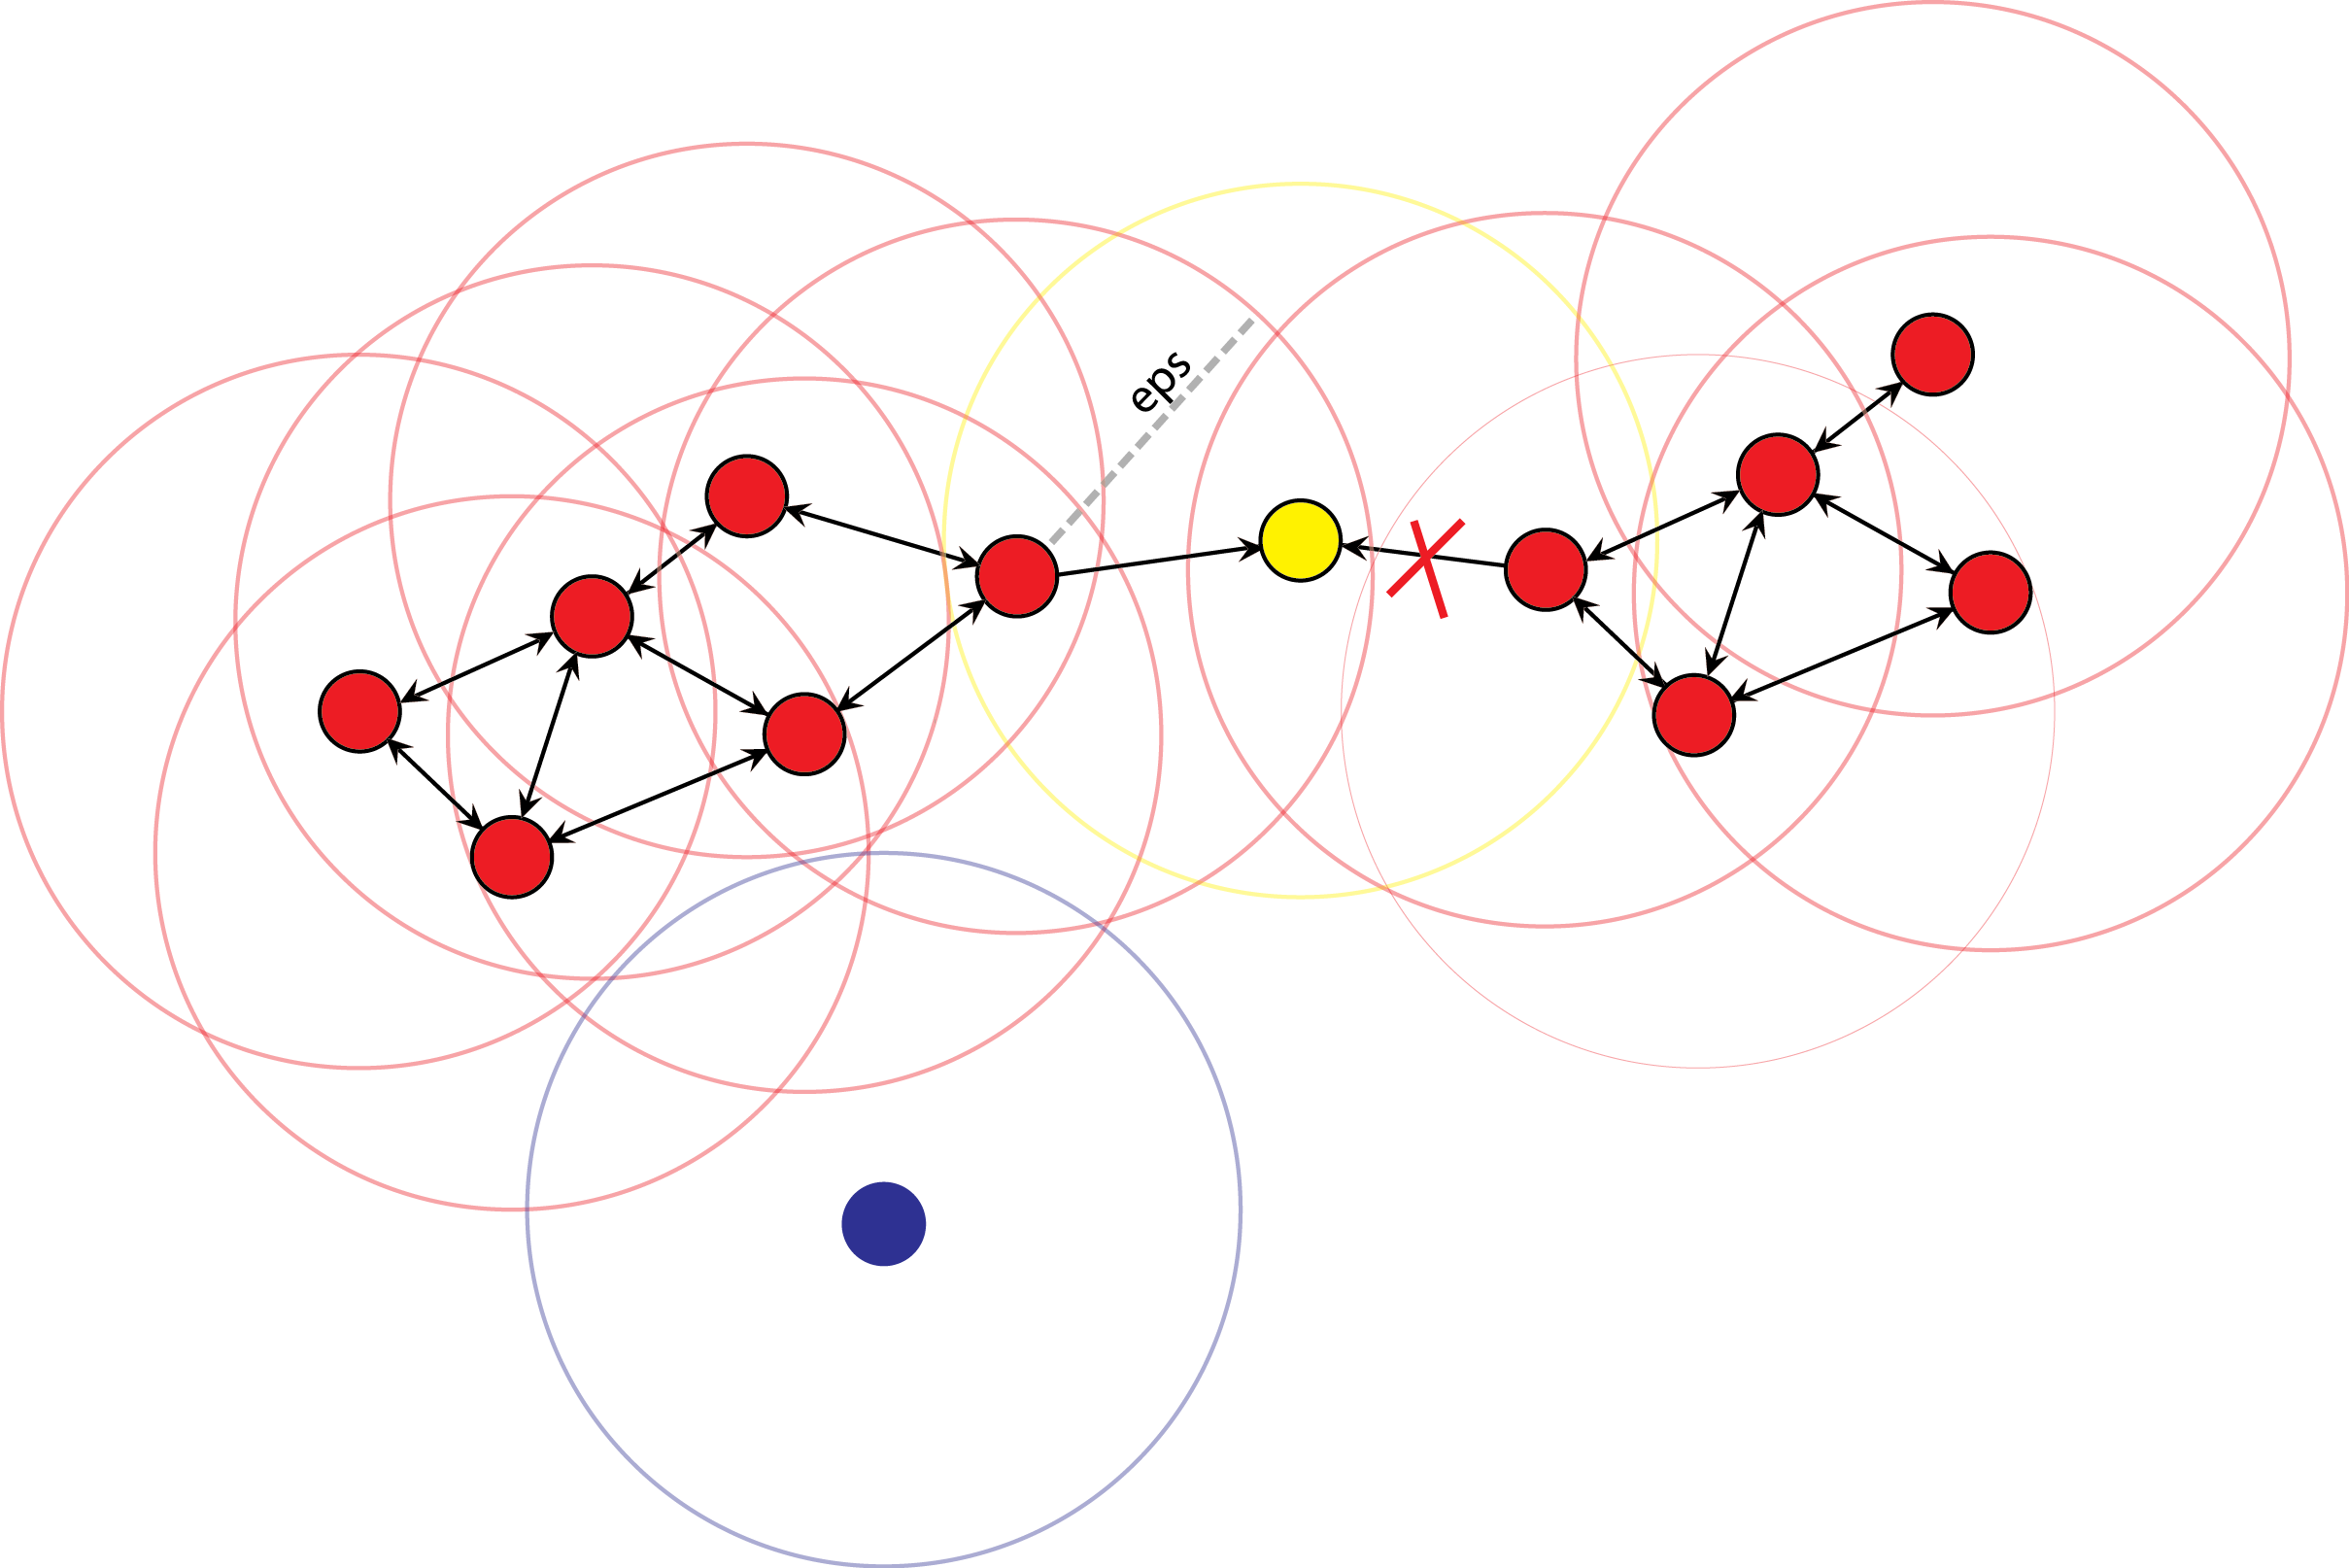
\includegraphics[width=0.6\textwidth]{dbscanRevisited}
\caption{border object density reachable da due core-object}
\label{fig:dbscanGraphRevisited}
 \end{figure}
%density connected def
 
 


\section{Sensitive Hashing}
Un problema fondamentale che molti task di Data Mining devono affrontare è quello di esaminare i dati per trovare item "simili". Molto spesso questo problema è risolto cercando il Nearest Neighbor ( o i primi k-nearest neighbor) di un oggetto in qualche spazio metrico $R^d$ .
Nel caso di poche dimensioni (d=2, d=3) questo problema, si riesce a risolvere in maniera piuttosto efficiente (O(log n)) mediante l'utlizzo di strutture dati come K-D-Tree o R-tree che partizionano lo spazio delle feature. Tuttavia al crescere delle dimensioni (curse of dimensionality), queste strutture basate sul partizionamento dello spazio, degradano in una ricerca lineare \cite{Weber:1998:QAP:645924.671192} passando quindi ad una complessità quadratica.
Per rendere meglio l'idea supponiamo di voler calcolare i documenti più simili in una collezione composta da un milione di documenti, si avrebbero quindi  $\binom{100000}{2}$  coppie di cui calcolare la similarità. Se ci si impiega un microsecondo per ogni calcolo di similarità, sarebbero necessari quasi sei giorni per valutare tutte queste coppie.
Se l'obiettivo è proprio il calcolo delle similarità di ogni possibile coppia, l'unico modo per ridurre il tempo necessario è usare una qualche forma di parallelismo. Tuttavia spesso, come nel caso del NNS-problem, si è interessati solo alle coppie più simili o più in generale a quelle coppie la cui similarità è al di sopra di una determinata soglia. \'E quindi sufficiente considerare solo quelle coppie che "probabilmente" sono simili, piuttosto che considerarle tutte. Proprio a tale scopo, se la dimensionalità dei dati è piuttosto alta, è possibile usare la tecnica del \emph{Local Sensitive Hashing} (LSH) \cite{Lsh} \cite{Gionis:1999}. L'idea chiave dell'LSH è quella di eseguire l'hasing dei punti attraverso molte funzioni di hashing, in modo tale che per ogni funzione la probabilità di collisione sia più alta per i punti vicini fra loro, rispetto ai punti più distanti.
Dopo aver eseguito l'hashing  tutte le coppie che sono state mappate nello stesso "bucket" possono essere considerate come \emph{coppie candidate}, solo queste coppie saranno valutate per determinare quali sono realmente simili. Quello che ci si augura è che, le coppie di item fra loro dissimili non vegano mai mappate verso lo stesso bucket,tali coppie rappresentano infatti dei \emph{false positive}. Allo stesso tempo ci si auspica che tutte (o la maggior parte) delle coppie realmente simili siano mappate nel medesimo bucket, le coppie che simili che non sono ricadute nello stesso bucket rappresentano i \emph{false-negative}
\subsection{Teoria dell'LSH}
 L'LSH è un framework per costruire strutture dati che permettono di ricercare i "near neighbor" all'interno di una collezione di vettori altamente dimensionali.  Dato un insieme $P$ contenente vettori D-dimensionali, l'obiettivo è di costruire una struttura che consenta di ritrovare, per un qualsiasi query point $q$, tutti quei punti che giacciono in un raggio di distanza $cR$ (dove $c$ rappresenta un fattore di approssimazione $>1$), o più formalmente gli \emph{R-near neighbors} di q.
 Data una funzione di hashing $h$ diremo che una coppia di oggetti $(x,y)$ sarà una \emph{candidate}   se $h(x)=h(y)$. Sia $d(\cdot,\cdot)$ una qualche funzione  definita su un insieme di oggetti $S$
\begin{definizione}[Locality-sensitive hashing] 

Una famiglia di funzioni $H$ si dice $(d_1,d_2,p_1,p_2)-Sensitive$ se  $\forall (x,y) \in S ,\;\forall h \in H $ 


\begin{itemize}
\item $se \quad  d(x,y)\leq d_1 \Rightarrow P_H[h(x)==h(y)]\geq p_1  $,
\item $se \quad  d(x,y)\geq d_2 \Rightarrow P_H[h(x)==h(y)]\leq p_2  $
\end{itemize}
dove $p_1>p_2$
\end{definizione}
A differenza di algoritmi di hashing classici dove si cercano di evitare delle collsioni per item diversi, in questo caso si cerca di massimizzare la probabilità di collisione per item vicini.
Dato un oggetto $q$ come query, verranno restituiti gli oggetti che giacciono nello stesso bucket $h(q)$
 

\begin{figure}[h]
\centering
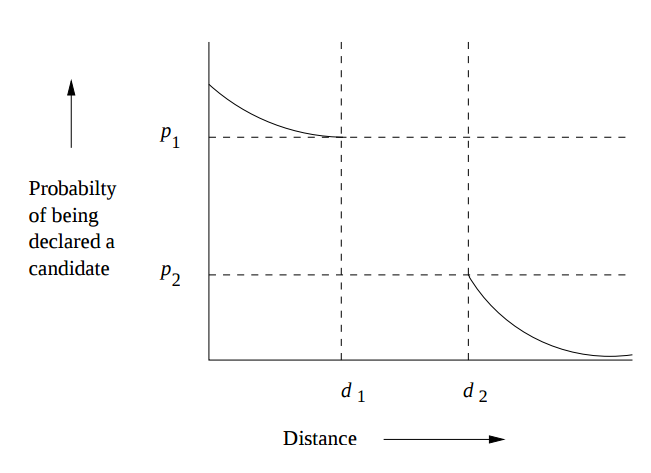
\includegraphics[width=0.6\textwidth]{hashFamily.png}
\caption{esempio di una funzione $(d_1,d_2,p_1,p_2)-sensisitve$}
\label{fig:lshfamily}
\end{figure} 
 
La figura \ref{fig:lshfamily} mostra un la probabilità che una possibile funzione di una famiglia  $(d_1,d_2,p_1,p_2)-sensisitve$ dichiari una coppia come candidata.

Data una famiglia di funzioni hash $(d_1,d_2,p_1,p_2)-sensisitve$ \emph{H} si può costruire una nuova famiglia di funzioni \emph{H'} applicando la \emph{AND-construction} su H come segue: ciascuna funzione di H' sarà data dalla concatenazione  da $r$ funzioni di H : $\lbrace h_1....h_r \rbrace $. Allora per ogni funzione $h$ in \emph{H'} diremo che: $h(x)=h(y)$ se $h_i(x)=h_i(y)$ per ogni $i...r$.  Dato che le funzioni $h_i$ sono scelte in maniera indipendente da $H$, possiamo asserire che \emph{H'} è una famiglia $(d_1,d_2,p_1^r,p_2^r)-sensisitve$.
Se invece costruiamo una nuova famiglia di funzione, per mezzo di una disgiunzione di \emph{b} elementi  di \emph{H} (\emph{OR-construction}), passeremo da una famiglia  $(d_1,d_2,p_1,p_2)-sensisitve$ ad una  $(d_1,d_2,1-(1-p_1)^b,1-(1-p_2)^b)-sensisitve$ \emph{H'}. In questo caso diremo che: $h(x)=h(y)$ se esiste  un valore di $i$ tale che $h_i(x)=h_i(y)$ 
Se $p$ è la probabilità che elemento di \emph{H} dichiari una coppia $(x,y)$ come candidata, allora $1-p$ è la probabilità che non lo sia. Avendo $b$ funzioni $h_1,...,h_b$ avremo che la probabilità che nessuna di esse dichiari la coppia come candidata, pari a   $(1-p)^b$ , e di conseguenza $1-(1-p)^b$ sarà la probabilità che almeno una fra le $b$ funzioni dichiarerà la coppia come candidata.
\'E facile notare che la \emph{And-Construction} fa decrescere tutte le probabilità, mentre la \emph{OR-construction} ha l'effetto opposto.\'E però possibile, applicare in cascata queste due tecniche AND,OR in modo tale che la probabilità $p_2$ sia più bassa possibile, mentre $p_1$ sia quanto più possibile vicino ad 1, ottenendo a una famglia $(d_1,d_2,1-(1-p_1^r)^b,1-(1-p_2^r)^b)-sensisitve$. Scegliendo in maniera accurata i valori di $r$ e di $b$ sarà possibile controllare l'andamento della funzione di probabilità $1-(1-p^r)^b$.
Tale funzione, una volta fissati i parametri $r$ e $b$, descrive una \emph{S-curve}. Come per qualsiasi \emph{S-curve}, è possibile determinare il punto fisso, ovvero quel valore di $t$ che rimane inalterato dopo aver applicato, la funzione $p=1-(1-p^r)^b$. Tale valore può essere approssimato come $t\approx (1/b)^\frac{1}{r}$. Al di sotto di tale soglia, il valore di probabilità decresce,al di sopra cresce.Quindi, se  se scegliamo la probabilità più alta $p_1$ al di sopra della soglia $t$, e $p_2$ al di sotto, avremo che il valore  $p_2$ è ridotto e al contempo il valore $p_1$ viene innalzato. Bisogna quindi impostare i valori di $b,r$ in modo tale che il punto fisso della funzione, corrisponda proprio al valore di similarità tale per cui due elementi li possiamo considerare "simili".
\begin{figure}
    \centering
    \begin{subfigure}[b]{0.45\textwidth}
        \centering
        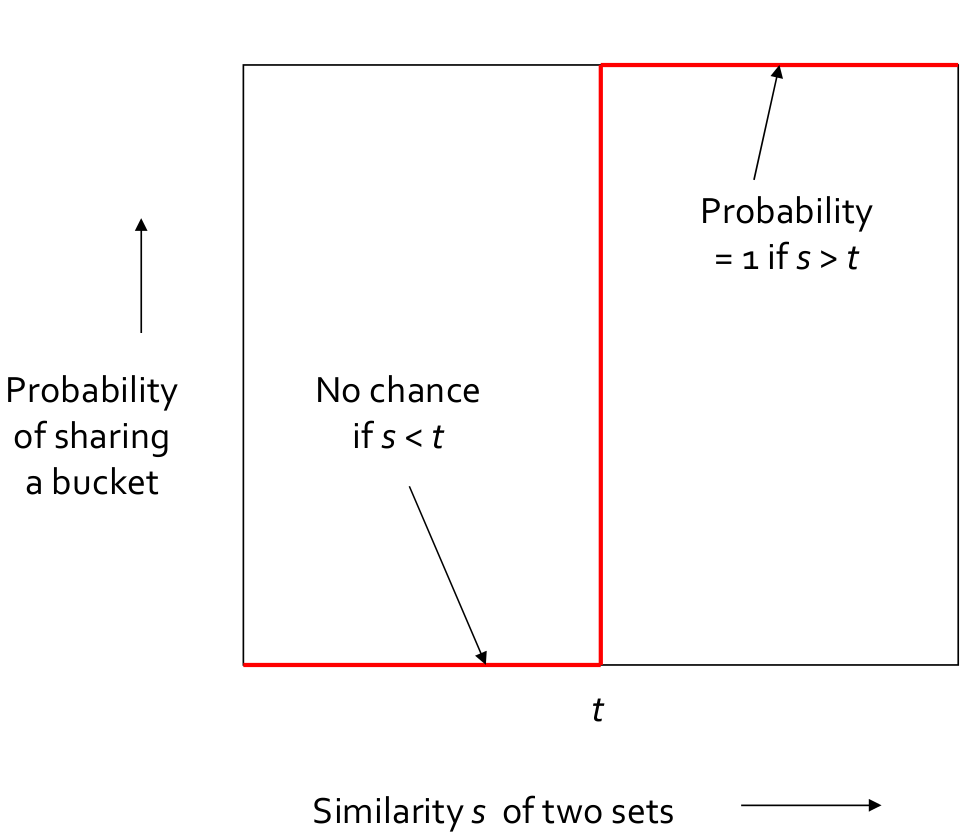
\includegraphics[width=\textwidth]{perfectSCURVE}
        \caption{s-curve ideale}
        \label{fig:perfectScurve}
    \end{subfigure}
    \hfill
    \begin{subfigure}[b]{0.45\textwidth}
        \centering
        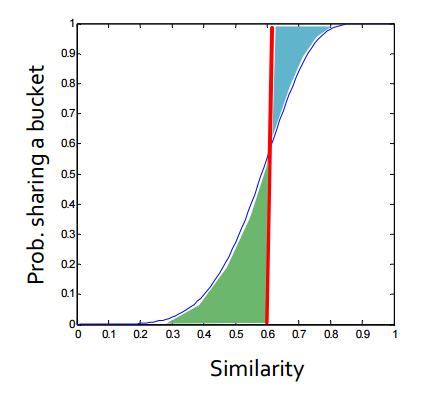
\includegraphics[width=\textwidth]{s-curve}
       \caption{s-curve r=5,b=10}
        \label{fig:realscurve}
    \end{subfigure}
    \hfill
    
    \caption{esempi di S-Curve}
    \label{fig:scurve}
\end{figure} 
La figura \ref{fig:perfectScurve}  mostra il caso ideale: dopo un valore di soglia la propabilità che due una coppia diventi candidata diviene immediatamente pari a 1, al di sotto pari a zero. Nella figura \ref{fig:realscurve} viene mostrato invece il caso in cui $r=5,b=10$, l'area verde indica il false-positive rate, mentre l'area blue indica il false negative rate.
Bisogna quindi, effettuare un tuning dei parametri $b,r$ per cercare di ritrovare la maggior parte delle coppie di elementi realmente simili, e al contempo avendo pochi false-positive.
Bisogna tenere a mente, però , che i false-positive possono essere filtrati con una fase di post-processing valutando la similarità reale fra le coppie restituite, i false negative, invece non possono essere in alcun modo recuperati, poiché rappresentano quelle coppie di item la cui distanza è bassa, ma che non sono state mappate nello stesso bucket.
\bibliographystyle{plain}
\subsection{LSH-Cosine}
In questo lavoro di tesi poiché si stanno analizzando documenti testuali, verrà utilizzata una famiglia di funzioni di hashing local-sensitive per la distanza del coseno. In particolare sarà adottato lo schema di lsh proposto da Charikar\cite{Charikar:2002:SET:509907.509965} in cui la   la probabilità che due punti collidano (ovvero che siano mappati verso lo stesso bucket), è proporzionale al coseno dell'angolo fra di loro. Data una collezione di vettori in $R^d$ viene definita una famiglia di funzioni hashing come segue: si sceglie un vettore random $\vec{r}$ le cui componenti sono presse da una distribuzione Gaussiana. Proprio grazie a questo vettore random verrà definita una funzione di hashing come segue:
\begin{equation}
\label{eq:hashRandom}
h_{\vec{r}}(\vec{u}):=\begin{cases}
1& \text{se  $\vec{r}\cdot \vec{u}\geq0$,}\\
0& \text{se  $\vec{r}\cdot \vec{u}\leq0$,}\\
\end{cases}
\end{equation}
La figura \ref{fig:hashingFunction} mostra l'interpretazione geometrica dell'equazione \ref{eq:hashRandom}, ovvero valutare il segno del prodotto interno fra il vettore che definisce la funzione di hashing, e un un vettore item, equivale a stabilire se 
l'item è al di sotto o al di sopra dell'iperpiano identificato dalla funzione.
Costruendo in questa maniera una funzione di hashing si avrà che, per due vettori $\vec{u},\vec{v}$,
\begin{equation}
\label{eq:probhash}
P[h_{\vec{r}}(\vec{u})=h_{\vec{r}}(\vec{v}))]=1-\frac{\theta(\vec{u},\vec{v})}{\pi}
\end{equation} 
Secondo il teorema\ref{eq:probhash} \cite{Goemans:1995:IAA:227683.227684},  la probabilità che un iperpiano random, separi due vettori è direttamente proporzionale all'angolo fra di essi. 
\begin{figure}
    \centering
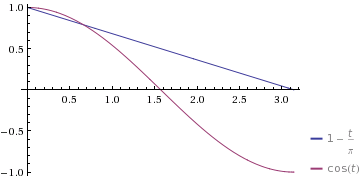
\includegraphics[width=0.6\textwidth]{cosineLSH}
\caption{approsimazione sim. coseno}
\label{fig:cosApprox}
\end{figure} 
In figura \ref{fig:cosApprox} si può notare che per piccoli angoli (non vicini all'angolo retto),  $ 1 - \frac{\theta}{\pi}$ è una buona approssimazione per  $\cos(\theta)$. Inoltre, dall'equazione \ref{eq:probhash} si ha che 
\begin{equation}
cos(\theta(u,v))=cos((1-P[h_r(u)=h_r(v)])\pi)
\end{equation}
Grazie a questa equazione, è possibile stimare la probabilità del coseno attraverso il risultato dell'applicazione delle funzioni di hashing. Guardando con più attenzione si può notare che
\begin{equation*}
 P[h_r(u)=h_r(v)])=g1-hammingDistance(h_r(u),h_r(v))/r
\end{equation*}
In pratica, questa uguaglianza permette di passare dal problema del calcolo della similarità del coseno fra due vettori altamente dimensionali, al problema del calcolo della distanza di hamming fra due stringhe.

 Anche questa famiglia di funzioni di hashing può essere aplificata con la tecnica AND-OR precedentemente descritta.
\begin{figure}
    \centering
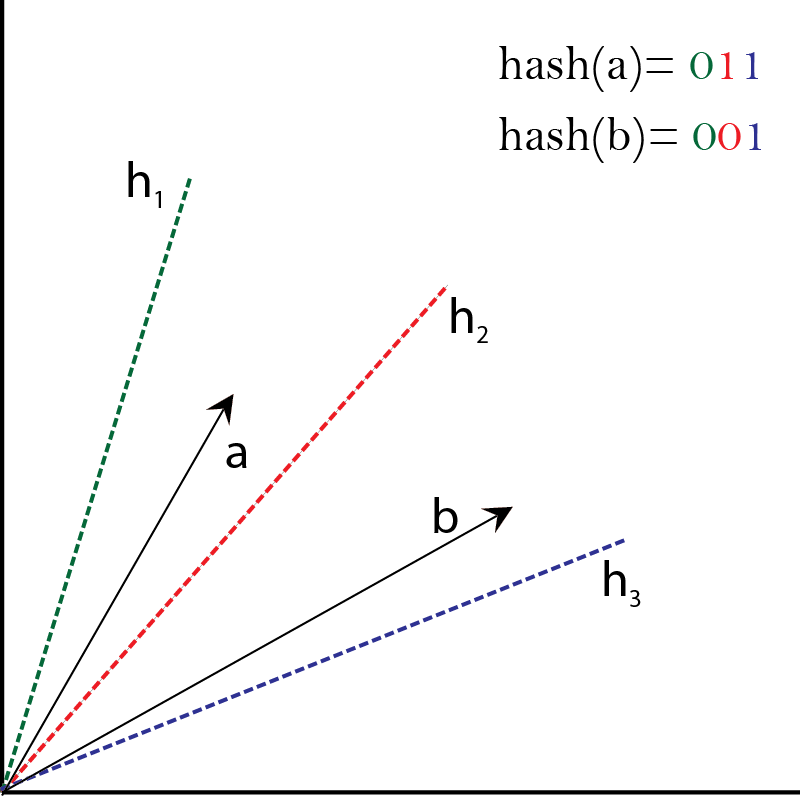
\includegraphics[width=0.5\textwidth]{hashing}
\caption{funzione di hashing}
\label{fig:hashingFunction}
\end{figure} 

 